\documentclass{article}
% NeurIPS 2026 workshop submission (single blind).
\usepackage[sglblindworkshop]{neurips_2026}

\usepackage[utf8]{inputenc}
\usepackage[T1]{fontenc}
\usepackage{hyperref}
\usepackage{url}
\usepackage{booktabs}
\usepackage{amsfonts}
\usepackage{amsmath}
\usepackage{amssymb}
\usepackage{nicefrac}
\usepackage{microtype}
\usepackage{xcolor}
\usepackage{graphicx}
\usepackage{amsthm}
\usepackage{tikz}
\usetikzlibrary{arrows.meta, positioning, fit, calc}

\newtheorem{theorem}{Theorem}
\newtheorem{proposition}{Proposition}
\newtheorem{assumption}{Assumption}

\newcommand{\method}{CP-IRL}

\title{From Inverse Optimization to Sequential Decisions:\\
Conformal Prediction for Inverse Reinforcement Learning}

\author{%
  Yuhan Chi \\
  Fudan University \\
  \texttt{yhchi25@m.fudan.edu.cn} \\
}

\begin{document}

\maketitle

\begin{abstract}
Inverse reinforcement learning (IRL) is inverse optimization with a sequential
forward problem: demonstrations reveal an unknown reward, which is then
optimized to prescribe a policy. Seen this way, IRL inherits a weakness that
Conformal Inverse Optimization (CIO) identified for one-shot decisions --
collapsing a heterogeneous population of demonstrators to one reward point
estimate can produce an arbitrarily bad policy. We introduce \textbf{\method{}},
which transfers CIO's calibrate-then-robustify principle to Markov decision
processes: from a population of demonstrators, \method{} conformally calibrates
a set of reward parameters consistent with a new demonstrator, then optimizes a
policy against that ambiguity. Two pieces of new machinery make this tractable.
First, the Bellman resolvent reduces each calibration score to a
reward-dimensional (rather than reward-plus-value-function-dimensional) convex
program. Second, we show the robust MDP is convex whenever ambiguity is
confined to the reward and the transition kernel is fixed -- for any compact
ambiguity set -- and that this boundary is tight: a two-state counterexample
loses convexity the moment ambiguity also touches the dynamics. Building on
this machinery, we prove finite-sample coverage, a regret bound, and a
separation result where point-estimate IRL's regret grows without bound while
\method{}'s vanishes. Experiments on random MDPs, gridworld, and Objectworld
then locate the method's actual scope: robust hedging cuts true-reward regret
under systematic estimation bias, but costs regret when the point estimate is
merely noisy and already unbiased.
\end{abstract}

\section{Introduction}

Inverse reinforcement learning (IRL) is usually introduced as its own problem:
infer a reward from behavior, then optimize that reward to get a policy. But
end to end, IRL is a sequential instance of \emph{inverse optimization} -- the
observed decision is a policy or trajectory, the latent objective is a reward
function, and the forward problem is an MDP. Under that view, uncertainty about
the recovered reward should propagate into the downstream decision instead of
being discarded once a point estimate is fit.

Conformal Inverse Optimization (CIO) builds exactly this pipeline for one-shot
decisions~\cite{lin2024conformal}: it replaces a single recovered objective
with a conformally calibrated uncertainty set and optimizes robustly over that
set, with a finite-sample, distribution-free guarantee under exchangeability.
CIO's own separation example shows the stakes -- point-estimate inverse
optimization can carry unbounded downstream regret even with unlimited data.
This raises the question we answer here: can CIO's calibrate-then-robustify
principle transfer to inverse reinforcement learning without losing coverage
or tractability?

Our answer, \method{}, keeps CIO's pipeline and rebuilds its machinery for
sequential decisions. A population of demonstrators supplies the exchangeable
calibration units; each observed policy defines a feasible reward set through
Bellman optimality; split conformal prediction calibrates a spherical cap
around an IRL point estimator; a robust MDP turns the calibrated ambiguity
into a deployed policy. Two obstacles block a direct transplant of this
template from LPs to MDPs. First, CIO's per-point calibration score is
computable in closed form because the forward problem is a linear program, so
reward feasibility reduces to LP dual feasibility. An MDP has no such
shortcut: ``this policy is optimal for this reward'' is a Bellman-optimality
condition, and checking it naively means jointly optimizing over the reward
\emph{and} the policy's value function, a variable count that grows with the
state space. Second, CIO's robust forward problem is a single robust linear
program, but the MDP analogue is a minimax game over policies,
$\max_\pi\min_\theta$, over an ambiguity set -- and robust MDPs with ambiguity
that couples across states are NP-hard in general~\cite{wiesemann2013robust},
with tractable results typically relying on \emph{rectangularity} assumptions
that restrict how the adversary can vary its choice by state.

We resolve both obstacles. Figure~\ref{fig:pipeline} lays out the transfer:
same calibrate-then-robustify template on both rows, with the two obstacles
resolved where the sequential setting departs from CIO's one-shot LP. The
contributions are:

\begin{figure}[t]
  \centering
  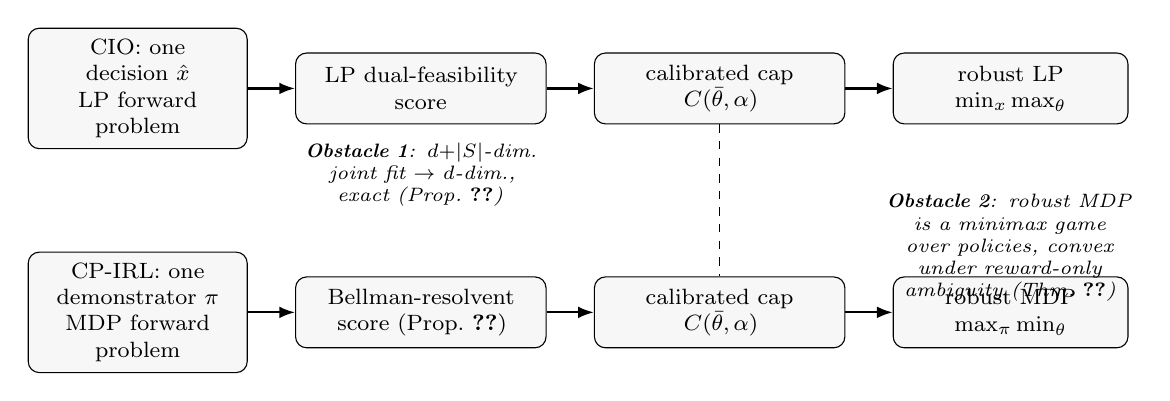
\begin{tikzpicture}[
      box/.style={draw, rounded corners, align=center, minimum height=0.9cm,
        font=\footnotesize, fill=black!3, inner sep=4pt},
      lbl/.style={font=\scriptsize\itshape, align=center, text width=3.1cm},
      arr/.style={-{Latex[length=2mm]}, thick},
      node distance=6mm
    ]

    \node[box, text width=2.5cm] (cio-in)  {CIO: one decision $\hat x$\\LP forward problem};
    \node[box, text width=2.9cm, right=of cio-in] (cio-score) {LP dual-feasibility\\score};
    \node[box, text width=2.9cm, right=of cio-score] (cap) {calibrated cap\\$C(\bar\theta,\alpha)$};
    \node[box, text width=2.7cm, right=of cap] (cio-out) {robust LP\\$\min_x\max_\theta$};

    \node[box, text width=2.5cm, below=13mm of cio-in]  (irl-in)  {\method{}: one demonstrator $\pi$\\MDP forward problem};
    \node[box, text width=2.9cm, right=of irl-in] (irl-score) {Bellman-resolvent\\score (Prop.~\ref{prop:resolvent})};
    \node[box, text width=2.9cm, right=of irl-score] (cap2) {calibrated cap\\$C(\bar\theta,\alpha)$};
    \node[box, text width=2.7cm, right=of cap2] (irl-out) {robust MDP\\$\max_\pi\min_\theta$};

    \draw[arr] (cio-in) -- (cio-score);
    \draw[arr] (cio-score) -- (cap);
    \draw[arr] (cap) -- (cio-out);
    \draw[arr] (irl-in) -- (irl-score);
    \draw[arr] (irl-score) -- (cap2);
    \draw[arr] (cap2) -- (irl-out);

    \node[lbl, above=1mm of $(cio-score)!0.5!(irl-score)$, yshift=-3mm] (l1)
      {\textbf{Obstacle 1}: $d{+}|S|$-dim.\ joint fit $\to$ $d$-dim., exact (Prop.~\ref{prop:resolvent})};
    \node[lbl, below=1mm of $(cio-out)!0.5!(irl-out)$, yshift=3mm] (l2)
      {\textbf{Obstacle 2}: robust MDP is a minimax game over policies, convex under reward-only ambiguity (Thm.~\ref{thm:convexity})};

    \draw[dashed] (cap.south) -- (cap2.north);
  \end{tikzpicture}
  \caption{The transfer at a glance. \method{} keeps CIO's calibrate-then-robustify
  template (same calibrated cap $C(\bar\theta,\alpha)$, dashed link) but replaces
  every sequential-specific piece: the nonconformity score (\S\ref{sec:method-calibration})
  and the robust decision problem (\S\ref{sec:method-robust}).}
  \label{fig:pipeline}
\end{figure}

\begin{itemize}
\item \textbf{Transfer: conformal inverse optimization for IRL.}
  We formulate one demonstrator as one exchangeable inverse-optimization
  instance, calibrate a reward uncertainty set through Bellman-optimal reward
  feasibility, and establish finite-sample coverage together with a
  true-reward regret bound (\S\ref{sec:setting}--\S\ref{sec:theory}).
\item \textbf{Optimization: sequential structure without state-sized calibration}
  (\S\ref{sec:method-calibration}). For a fixed demonstrator policy, the Bellman
  resolvent $(I-\beta P_\pi)^{-1}$ makes the induced value function
  \emph{linear} in the reward parameter -- the same identity underlying Ng \&
  Russell's~\cite{ng2000algorithms} feasible-reward characterization, which we
  repurpose as a calibration-score reduction. Substituting it shrinks the
  per-demonstrator calibration score from a joint optimization over $(\theta,V)$
  (size $d+|S|$) to one over $\theta$ alone (size $d$), exactly, by the policy
  improvement theorem. We also give a Sherman--Morrison--Woodbury update that
  recomputes the resolvent in $O(k^2|S|+k^3)$ rather than $O(|S|^3)$ when two
  demonstrators' policies differ at only $k$ states.
\item \textbf{Tractability: a boundary between reward and dynamics ambiguity}
  (\S\ref{sec:method-robust}). The robust MDP is a convex program in
  occupancy-measure space for any compact reward ambiguity set, with the
  transition kernel fixed -- a Bellman-recursion-free argument that extends the
  closest sufficiency-side result (Gadot et al.~\cite{gadot2024solving}, who
  solve the convex $L_p$-ball case via H\"older duality and policy gradient) to
  arbitrary compact sets. We show this boundary is tight: a two-state,
  two-action MDP with a one-dimensional ambiguity set coupling reward and
  transition probability breaks concavity, with a hand-verifiable
  rational-valued Jensen violation.
\item \textbf{Scope: robustness helps under bias, not noise alone.}
  Our sequential analogue of CIO's separation example proves classical
  point-estimate IRL's regret can diverge while the calibrated policy's regret
  vanishes. Across random MDPs, a region-based gridworld, and Objectworld,
  calibrated robust hedging reduces true-reward regret when the point estimate
  is \emph{systematically} biased (as our degenerate construction manufactures),
  and increases it when the estimate is merely noisy but unbiased -- a precise,
  falsifiable condition for when the method pays off, which we report as a core
  finding rather than bury as a limitation.
\end{itemize}

\section{Related Work}
\label{sec:related}

\textbf{Inverse optimization and its calibration.} Inverse optimization
recovers parameters of an optimization problem from observed decisions
(Ahuja \& Orlin~\cite{ahuja2001inverse}; Chan et al.~\cite{chan2018inverse}).
Classical formulations return a point estimate; more recent work constructs
data-driven uncertainty sets around it (Chenreddy, Bandi \&
Delage~\cite{chenreddy2022datadriven}; Sun, Liu \& Li~\cite{sun2023predictthencalibrate}),
but -- as Lin, Delage \& Chan~\cite{lin2024conformal} show -- none of these give
the specific guarantee we need: that the \emph{next} observed decision's true
parameter is covered with a stated confidence, distribution-free. Conformal
Inverse Optimization is the first to close this gap using split conformal
prediction~\cite{vovk2005algorithmic}, and is the paper this work directly
extends from one-shot decisions to MDPs.

\textbf{Feasible reward sets in IRL.} A separate line of work characterizes the
\emph{set} of rewards consistent with observed IRL data
(Poiani et al.~\cite{poiani2024suboptimal}; Lazzati \& Metelli~\cite{lazzati2025robustness};
Skalse et al.~\cite{skalse2022invariance}) and proves PAC-style bounds on
recovering it, using it directly as a robust-MDP ambiguity set. This line
shares our target object -- a feasible reward set characterized by
Bellman-optimality constraints -- but its guarantees are PAC bounds requiring a
generative model of demonstrator sub-optimality; ours require only
exchangeability of demonstrators, no assumption on the \emph{process} by which
any individual demonstrator deviates from optimality. The transfer question
this line raises -- whether a feasible reward set identified on one MDP
transfers to another (Schlaginhaufen \& Kamgarpour~\cite{schlaginhaufen2024towards})
-- is a genuinely open problem for our setting that we do not attempt to close
here (see \S\ref{sec:discussion}).

\textbf{Robust MDPs and the rectangularity boundary.} Robust MDPs with
ambiguity coupling across states are NP-hard in general
(Wiesemann, Kuhn \& Rustem~\cite{wiesemann2013robust}); tractability is
classically recovered via \emph{s-} or \emph{sa-rectangularity}
(Iyengar~\cite{iyengar2005robust}; Nilim \& El Ghaoui~\cite{nilim2005robust}),
which restricts the adversary to choose independently per state. Recent work
extends tractable, \emph{non}-rectangular ambiguity specifically for
reward-only uncertainty with a fixed transition kernel: Gadot et
al.~\cite{gadot2024solving} solve the convex $L_p$-ball case exactly via
H\"older duality and a policy-gradient method with proven convergence; Xu et
al.'s Group-Robust MDPs~\cite{xu2026learning} handle \emph{feature-wise}
(d-rectangular) ambiguity that couples both reward \emph{and} transition, at
the cost of restricting to that rectangular structure. Our sufficiency result
(\S\ref{sec:method-robust}) covers the same fixed-kernel, reward-only regime as
Gadot et al. but for an \emph{arbitrary} compact ambiguity set (not only
$L_p$-balls), via a direct occupancy-measure convex program rather than a
policy-gradient method; our necessity result -- an explicit demonstration that
convexity is lost the moment ambiguity couples into the kernel, even minimally
-- has no counterpart in either paper.

\textbf{Conformal prediction in RL-adjacent settings.} Conformal prediction has
been used for offline-RL pessimism from Q-value or state-action-coverage
uncertainty (UARM, Pan et al.~\cite{pan2026uncertaintyaware}), for calibrated
intervals in infinite-horizon policy evaluation, and for modeling \emph{other
agents' actions} as conformal prediction sets in multi-agent RL (CAMMARL,
Gupta \& Kahou~\cite{gupta2023cammarl}) -- the last of these is explicitly
motivated by an analogy to IRL but never calibrates a reward set. None combine
conformal calibration with a reward vector recovered from a population of IRL
demonstrators and a robust-MDP regret guarantee, which is the gap this paper
closes.

\textbf{Preference learning and RLHF.} Preference-based and RLHF-style learning
fits a reward (or policy) from labeled comparisons or demonstrations, typically
from individual expert trajectories (Christiano et al.~\cite{christiano2017deep};
Rafailov et al.~\cite{rafailov2023direct}) or crowdsourced preference
populations. Our per-demonstrator exchangeable-unit design (\S\ref{sec:setting})
is structurally suited to recast ``one annotator, one calibration point'' for
heterogeneous-preference RLHF populations. The resulting coverage guarantee is
in the intersection-nonemptiness sense of Theorem~\ref{thm:coverage}, not
parameter containment: the calibrated reward-ambiguity set is compatible with
a $\gamma$-fraction of the annotator population's individual reward functions,
which are never directly observed. We are not aware of this guarantee
elsewhere in the RLHF calibration literature, though we test it only on a toy
response-selection MDP, not at RLHF's actual scale (\S\ref{sec:discussion}).

\section{Setting}
\label{sec:setting}

We now make the CIO--IRL correspondence precise. We adopt the
population-of-demonstrators setting used throughout this work: a shared tabular
MDP $M = (S, A, P, \beta, \phi)$ with known transition kernel $P$, discount
$\beta$, and feature map $\phi: S \times A \to \mathbb{R}^d$ inducing reward
$r_\theta(s,a) = \phi(s,a)^\top\theta$. A population of demonstrators draws
perceived rewards $\hat\theta_1, \dots, \hat\theta_N \sim P_\theta$ i.i.d.\ and
each acts optimally in $M$ under their own $\hat\theta_k$, producing an observed
policy $\pi_k = \pi^*(\hat\theta_k)$ -- we assume the full deterministic policy
is observed exactly, not estimated from a finite trajectory sample; relaxing
this to trajectory-level observation would make $\hat\Theta(\pi_k)$ itself an
estimated (rather than exact) feasible set and is outside the scope of the
guarantees below.

\begin{assumption}[Exchangeable calibration unit]
\label{ass:unit}
The pairs $(\hat\theta_k, \pi_k)$, $k=1,\dots,N,N{+}1$, are i.i.d.\ (hence
exchangeable), and $M$ (in particular $P$) is shared and fixed across all
demonstrators and the deployment instance.
\end{assumption}

Under Assumption~\ref{ass:unit}, each demonstrator plays the role of one
(decision, context) pair in CIO's setting, and it is the setting under which
CIO's coverage argument transplants essentially verbatim
(\S\ref{sec:theory}, Theorem~\ref{thm:coverage}). We commit to this ``unit A''
design over two weaker alternatives -- per-task exchangeability with a single
demonstrator (still exchangeable, treated as an easy corollary) and
per-trajectory exchangeability within one demonstrator (broken by
within-trajectory Markov dependence, and used only as an ablation) -- and are
explicit throughout about what breaks under each relaxation.

The learning task, mirroring CIO's pipeline, has three steps: (i) split the
population into training and calibration sets; (ii) fit a point estimate
$\bar\theta$ on the training set with any IRL method (we use and compare a
sub-optimality-loss linear program, MaxEnt IRL, and Bayesian IRL by MCMC --
\S\ref{sec:experiments}); (iii) calibrate a spherical-cap uncertainty set
$C(\bar\theta, \alpha) = \{\theta : \|\theta\|_2 \leq 1,\ \theta^\top\bar\theta \geq
\cos\alpha\}$ on the calibration set and solve the robust MDP
$\max_\pi \min_{\theta \in C(\bar\theta,\alpha)} \theta^\top \mu(\pi)$ in
occupancy-measure space, where $\mu(\pi)$ is $\pi$'s occupancy measure.

\section{Method}

\subsection{Tractable calibration via the Bellman resolvent}
\label{sec:method-calibration}

CIO's calibration score for a validation point $k$ is
$c_k = \max_\theta \{\theta^\top\bar\theta : \theta \in \Theta^{\mathrm{OPT}}(\hat x_k, u_k), \|\theta\|_2 \leq 1\}$,
where $\Theta^{\mathrm{OPT}}$ is characterized by LP dual feasibility --
tractable because the forward problem is a linear program. In an MDP, the
analogous feasible set for a policy $\pi$ is
\[
\hat\Theta(\pi) = \{\theta : \|\theta\|_2 \leq 1,\ Q^\pi_\theta(s,a) \leq Q^\pi_\theta(s, \pi(s))\ \forall s, \forall a\},
\]
the exact set of reward vectors for which $\pi$ is Bellman-optimal, by the
policy improvement theorem. Computing this naively requires the joint
optimization $\max_{\theta,V} \theta^\top\bar\theta$ subject to the
Bellman-optimality inequalities written in terms of both $\theta$ and the a
priori unknown value function $V$ -- a variable count of $d + |S|$.

The key fact we use, which is the sequential-decision restatement of the
feasible-reward characterization of Ng \& Russell~\cite{ng2000algorithms}: for
a \textbf{fixed} policy $\pi$, the policy's own induced value function
$V^\pi_\theta$ is \emph{linear} in $\theta$, via the Bellman resolvent.

\begin{proposition}[Resolvent-based score reduction]
\label{prop:resolvent}
Fix a policy $\pi$, let $P_\pi \in \mathbb{R}^{|S|\times|S|}$ be the induced
state-transition matrix ($P_\pi(s,s') = P(s,\pi(s),s')$), and let $\Phi_\pi \in
\mathbb{R}^{|S|\times d}$ be the feature matrix restricted to the actions $\pi$
takes ($\Phi_\pi(s,\cdot) = \phi(s,\pi(s))^\top$). Let
$W_\pi := (I-\beta P_\pi)^{-1}\Phi_\pi$ (well-defined since $\beta \in [0,1)$). Then $V^\pi_\theta = W_\pi\theta$ and
$Q^\pi_\theta(s,a) = \Psi_\pi(s,a)^\top\theta$ with
$\Psi_\pi(s,a) := \phi(s,a) + \beta P(s,a,\cdot)^\top W_\pi$, both linear in
$\theta$. Consequently
\[
\hat\Theta(\pi) = \{\theta : \|\theta\|_2 \leq 1,\ \Psi_\pi(s,a)^\top\theta \leq \Psi_\pi(s,\pi(s))^\top\theta\ \ \forall s,a\},
\]
exactly (no relaxation), and the calibration score
$c_k = \max_{\theta \in \hat\Theta(\pi_k)} \theta^\top\bar\theta$ is an
optimization over $\theta$ alone -- size $d$, not $d+|S|$ -- with $W_{\pi_k}$
(and hence $\Psi_{\pi_k}$) precomputed once per distinct policy via a single
resolvent solve.
\end{proposition}

The proof substitutes the linear Bellman equation's solution into $Q^\pi_\theta$
and rewrites the policy-improvement optimality condition using $\Psi_\pi$;
full proof in Appendix~\ref{app:proof-resolvent}. We checked Proposition~\ref{prop:resolvent} against a slow joint-$(\theta,V)$
reference implementation and against independent value iteration, matching to
solver precision on randomized instances; the speedup over the joint
formulation grows with $|S|$, 2--5.5$\times$ at a few hundred states. The
Sherman--Morrison--Woodbury update -- recomputing the resolvent in
$O(k^2|S|+k^3)$ rather than $O(|S|^3)$ when a new demonstrator's policy
differs from an already-resolved one at only $k$ states -- has no counterpart
in Ng \& Russell~\cite{ng2000algorithms}; it is the piece specific to
calibrating against a whole population rather than a single demonstrator.

\subsection{A tight tractability boundary for the robust MDP}
\label{sec:method-robust}

The robust decision problem, $\max_\pi \min_{\theta \in C} \theta^\top\mu(\pi)$,
is a minimax game over policies. We work in occupancy-measure space: $M(P)$
denotes the (fixed, since $P$ is known) polytope of achievable occupancy
measures $\mu$, normalized so $\sum_{s,a}\mu(s,a)=1$, and
$\Phi \in \mathbb{R}^{|S \times A| \times d}$ is the matrix whose rows are
$\phi(s,a)^\top$ (matching the convention already used for $\Phi_\pi$ in
\S\ref{sec:method-calibration}), so that $\theta^\top\Phi^\top\mu = \sum_{s,a}
\mu(s,a)\, r_\theta(s,a)$ is the expected per-step reward of occupancy measure
$\mu$ under reward $\theta$, and $\theta^\top\Phi^\top\mu/(1-\beta)$ is the
corresponding expected discounted return. The robust objective is
$\max_{\mu \in M(P)} \min_{\theta \in C} \theta^\top\Phi^\top\mu$ (the
$1/(1-\beta)$ factor is a positive constant and does not affect the
$\arg\max$).

\begin{theorem}[Reward-only ambiguity is convex; this is tight]
\label{thm:convexity}
\textbf{(a) Sufficiency.} For \emph{any} nonempty compact ambiguity set
$C \subseteq \mathbb{R}^d$ (e.g., our calibrated spherical cap
$C(\bar\theta,\alpha) = \{\theta:\|\theta\|_2\le 1,\ \theta^\top\bar\theta \geq
\cos\alpha\}$, a cap of the unit ball rather than the unit sphere), if the
transition kernel $P$ is fixed and known, then
$\max_{\mu \in M(P)}\min_{\theta \in C}\theta^\top\Phi^\top\mu$ is a concave
maximization over the fixed compact polytope $M(P)$, hence a convex program.
\textbf{(b) Necessity.} This can fail as soon as ambiguity couples reward and
transition probability, even minimally: there exists a 2-state, 2-action MDP
and a convex, one-dimensional, non-product ambiguity set over $(\theta,P)$
jointly for which the analogous worst-case value function is not concave.
\end{theorem}

Part (a) holds because $g_C(x):=\min_{\theta\in C}\theta^\top x$ is concave
regardless of $C$'s shape and $M(P)$ does not depend on $\theta$; part (b)
exhibits an explicit rational-valued Jensen violation. Full proof, including
the closed-form counterexample, in Appendix~\ref{app:proof-convexity}. Part (a) generalizes the sufficiency result of Gadot et
al.~\cite{gadot2024solving} (who solve the convex $L_p$-ball case exactly via
H\"older duality and policy gradient) to an arbitrary compact $C$, via a direct
occupancy-measure argument. Part (b) shows the coupling required to break
concavity is minimal -- a single scalar $t$ linking reward and transition
ambiguity along a line segment, far short of a fully unconstrained
non-rectangular adversary -- and, to our knowledge, is not established by
either Gadot et al.\ or Xu et al.~\cite{xu2026learning}. Note that failure of
concavity is a failure of this \emph{particular} tractability argument, not by
itself a proof of NP-hardness; general non-rectangular robust MDPs are already
known to be NP-hard~\cite{wiesemann2013robust}.

\section{Theory}
\label{sec:theory}

Three more results follow, each the MDP/IRL analogue of a corresponding CIO
theorem: coverage, a regret bound, and separation. We spot-check each
computationally against the implemented solvers rather than trust the
derivation alone. A fourth item, efficiency, is an empirical measurement, not
a theorem.

\begin{theorem}[Coverage]
\label{thm:coverage}
Under Assumption~\ref{ass:unit}, let $\tau = \lceil(N_{\mathrm{val}}+1)\gamma\rceil$,
let $c_{(\tau)}$ be the $\tau$-th \emph{largest} calibration score among
$c_1,\dots,c_{N_{\mathrm{val}}}$ (Proposition~\ref{prop:resolvent}), and set
$\alpha_\gamma := \arccos(c_{(\tau)})$. Then
\[
\mathbb{P}\big(\hat\Theta_{\mathrm{new}} \cap C(\bar\theta, \alpha_\gamma) \neq \emptyset\big) \geq \gamma,
\]
where $\hat\Theta_{\mathrm{new}}$ is the new demonstrator's feasible reward
set. \textbf{This is an intersection-nonemptiness guarantee, not a containment
guarantee}: it does not by itself assert $\theta^*_{\mathrm{new}} \in
C(\bar\theta,\alpha_\gamma)$, only that the calibrated cap is compatible with
some reward for which $\pi_{\mathrm{new}}$ is optimal.
\end{theorem}

The proof transplants CIO's exchangeability argument line for line onto the
scores of Proposition~\ref{prop:resolvent} in place of CIO's LP dual scores
(Appendix~\ref{app:proof-coverage}). A marginal-coverage simulation against
the actual calibration code (150 trials per $(\gamma,N_{\mathrm{val}})$ cell)
confirms coverage $\geq\gamma$ at every tested combination; finite demonstrator
populations produce tied (atomic) calibration scores, the likely source of the
mild over-coverage we observe beyond the rank argument's
$1/(N_{\mathrm{val}}+1)$ slack (\S\ref{sec:experiments}).

\begin{theorem}[Regret bound]
\label{thm:regret}
Let $\|\phi\|_{2,\infty} := \max_{s,a}\|\phi(s,a)\|_2$,
$\nu(\mu) := \|\Phi^\top\mu\|_2/(1-\beta) \leq \bar\nu :=
\|\phi\|_{2,\infty}/(1-\beta)$ for any occupancy measure $\mu \in M(P)$ (a
Lipschitz constant for $\theta \mapsto \theta^\top\Phi^\top\mu/(1-\beta)$ in
$\theta$, via Cauchy--Schwarz), and let $\mu_{\mathrm{CIRL}}$, $\mu^*$ denote
the occupancy measures of the robust policy and of the true optimum
$\pi^*(\theta^*_{\mathrm{new}})$, respectively. Suppose the calibrated cap
$C(\bar\theta,\alpha_1)$ satisfies the \emph{almost-sure-covering} condition
$\mathbb{P}(\hat\Theta_{\mathrm{new}} \cap C(\bar\theta,\alpha_1) \neq \emptyset) = 1$
for a fresh demonstrator (strictly stronger than Theorem~\ref{thm:coverage}'s
$\gamma$-coverage; achievable trivially by taking $C$ to be the whole unit
ball, i.e.\ $\alpha_1$ at its maximal value, but then uninformative), that any
two unit-norm rewards optimal for the same policy are within $\eta$ of each
other (bounded feasible-set diameter), and that the population mean reward is
within $\sigma$ of $\theta^*_{\mathrm{new}}$ in $\ell_2$. Then the
\textbf{average optimality gap} $\mathrm{AOG} :=
V_{\theta^*_{\mathrm{new}}}(\mu^*) - V_{\theta^*_{\mathrm{new}}}(\mu_{\mathrm{CIRL}})$
(the true-reward regret of the robust policy relative to the in-hindsight
optimum) satisfies
\[
\mathrm{AOG} \leq \big(2\sin\alpha_1+\eta+\sigma\big)\,\nu(\mu^*) + (\eta+\sigma)\,\nu(\mu_{\mathrm{CIRL}}),
\]
and substituting the uniform bound $\bar\nu$ for both $\nu(\mu^*)$ and
$\nu(\mu_{\mathrm{CIRL}})$ gives the fully distribution-free corollary
$\mathrm{AOG} \leq (2\sin\alpha_1+2\eta+2\sigma)\,\bar\nu$.
\end{theorem}

The proof telescopes three terms -- Lipschitz continuity of
$\theta\mapsto\theta^\top\Phi^\top\mu$, a chord-length bound on
$C(\bar\theta,\alpha_1)$, and the robust policy's minimax optimality --
re-derived for the MDP's $\max_\pi\min_\theta$ sign convention rather than
transplanted from CIO's $\min_x\max_\theta$ one (Appendix~\ref{app:proof-regret}).
We checked $\bar\nu$ as a valid uniform Lipschitz constant against 200
randomized MDPs (zero violations) and confirmed the bound's numeric validity
directly on random instances.

This bound is loose, and we say so plainly. Cross-checked against the exact
closed-form regret for our degenerate construction below (where the
almost-sure-covering condition already holds at $\alpha_1=0$), the general
bound's looseness \emph{grows} with the construction's scaling parameter --
from roughly 8--15$\times$ at the low end of the tested range to roughly
390--430$\times$ at the high end, since the exact regret decays to zero while
$\eta,\sigma,\bar\nu$ converge to nonzero constants. CIO's own Example 1 bound
stays within a fixed 2.3--4$\times$ over the same kind of comparison, because
its construction keeps a richer feasible region that does not saturate this
way; ours grows.

\begin{theorem}[Separation]
\label{thm:separation}
There exists a single-state, two-action MDP (the sequential-decision analogue
of CIO's degenerate Example 1, with reward features the \emph{negation} of
CIO's original cost features) and an IRL point estimator such that: the
point-estimate solution converges to a degenerate direction
$\theta_u = (1,u)/\sqrt{1+u^2} \neq \theta^*$ (a unit vector, hence on the
boundary of the unit ball that $C(\bar\theta,\alpha)$ is a cap of) as the
scaling parameter $u\to\infty$, giving classical point-estimate IRL true-reward regret that grows
without bound in $u$; while the calibrated robust policy's regret is bounded
and shrinks to zero over the same range. The robust optimum is a genuine
mixture, with exact closed form $p^*(u) = u^2/(1+u^2)$, independent of the
calibration angle.
\end{theorem}

Theorem~\ref{thm:separation} is proved via Sion's minimax theorem applied to
the mixture's closed form (Appendix~\ref{app:proof-separation}), and
independently re-verified against the actual implemented solver to
$10^{-6}$ precision. Figure~\ref{fig:separation} shows the live 10-seed
computational confirmation. This separation exhibits the LP-based point
estimator's failure mode specifically (a degenerate boundary direction under
tie-breaking); \S\ref{sec:experiments} Q3 reports that MaxEnt and Bayesian IRL
do \emph{not} exhibit it on this same construction, and explains why.

\begin{figure}[t]
  \centering
  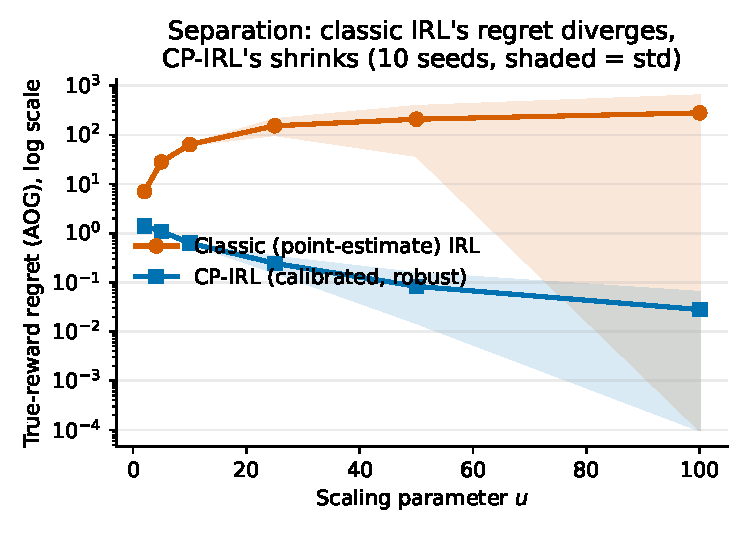
\includegraphics[width=0.6\linewidth]{figures/fig1_separation.pdf}
  \caption{Separation result (Theorem~\ref{thm:separation}): true-reward regret
  of the deployed policy, measured against the ground-truth reward
  $\theta^*_{\mathrm{new}}$, vs.\ the scaling parameter $u \in [2,100]$ (log
  scale), 10 seeds, shaded regions show $\pm 1$ std. ``Classic IRL'' is the
  sub-optimality-loss linear-program point estimator (\S\ref{sec:experiments}),
  which converges to the degenerate direction $\theta_u$; its regret (orange)
  grows monotonically and without bound. \method{}'s regret (blue) shrinks
  monotonically toward zero over the same range. Variance grows with $u$ for
  both curves, consistent with tie-breaking sensitivity as $\bar\theta$
  approaches the exact degenerate boundary.}
  \label{fig:separation}
\end{figure}

\textbf{Efficiency.} We confirm, empirically, that the calibrated set is not
vacuously wide: with a \emph{unified} noise parameter controlling all sources of
demonstrator population variation simultaneously, the calibrated angle shrinks
monotonically from $27.7^\circ$ to effectively $0^\circ$ as demonstrator-population
noise vanishes.

\section{Experiments}
\label{sec:experiments}

Three questions organize the experiments: \emph{(Q1)} does calibration hit its
target coverage without becoming vacuous; \emph{(Q2)} when does
robustification actually improve downstream regret; \emph{(Q3)} do the
conclusions hold beyond one IRL estimator or environment? We evaluate three
point estimators (a sub-optimality-loss linear program, MaxEnt IRL, and
Bayesian IRL via Metropolis--Hastings), each combined with three decision
rules (the plain point estimate, our calibrated robust policy, and a
``concentration baseline'' whose radius comes from a DKW concentration bound
instead of an exact conformal quantile), across three environments: random
tabular MDPs, a region-based gridworld with Voronoi reward features, and
Objectworld, the standard smooth-feature IRL benchmark.

The headline Q1--Q3 numbers use $|S|\le36$, $d\le5$, sized to run on a laptop
(20 CPU cores, no GPU, no commercial solver). To check this scale is not
load-bearing, we reran the full gridworld pipeline at $|S|=225$, $d=7$ --
6.25$\times$ more states, 2 more reward dimensions -- and confirmed the
pipeline stays under 35 seconds per demonstrator population up to $|S|=400$,
$d=8$. Q2's finding is unchanged at $|S|=225$: conformal-robust regret still
exceeds the plain estimate's for all three estimators (LP-IRL
$1.03\to3.19$, MaxEnt $1.01\to2.88$, Bayesian $0.06\to0.36$). We make no claim
beyond tabular MDPs; function approximation and language-model settings are
untested.

\textbf{Q1: coverage tracks the target.} Realized coverage tracks $\gamma$ in
every environment and estimator tested ($\sim$0.88--0.89 at $\gamma=0.8$ on
the gridworld), and the calibrated angle responds sensibly to $\gamma$,
demonstrator noise, and the train/calibration split. DKW is measurably looser
than exact conformal calibration at matched confidence, everywhere tested.

\begin{figure}[t]
  \centering
  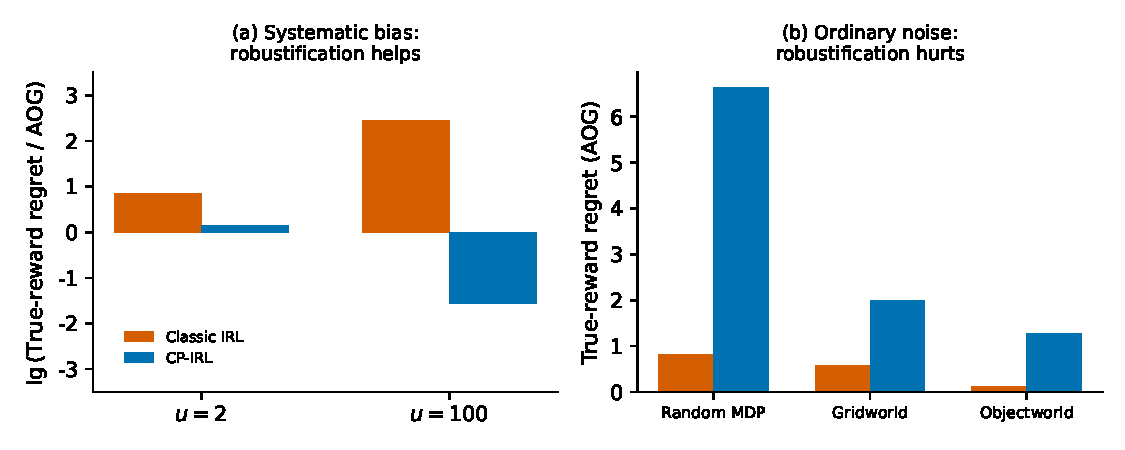
\includegraphics[width=\linewidth]{figures/fig2_insurance.pdf}
  \caption{The Q2 scope condition. \textbf{(a)} On the degenerate construction
  of Theorem~\ref{thm:separation} (log scale), robust hedging cuts true-reward
  regret by $5$--$10{,}000\times$ as $u$ grows from 2 to 100. \textbf{(b)} On
  three generic environments with ordinary, unbiased demonstrator noise (LP-IRL,
  $\gamma=0.8$), robust hedging instead \emph{costs} regret in every case. Same
  mechanism (worst-case hedging over a calibrated cap), opposite outcome,
  depending only on whether the point estimate is systematically biased.}
  \label{fig:insurance}
\end{figure}

\textbf{Q2: the benefit depends on systematic bias, not noise.}
Figure~\ref{fig:insurance} makes this concrete. On the degenerate construction,
where the point estimate is biased by construction, robust hedging cuts
true-reward regret sharply. On all three generic environments, under ordinary
demonstrator noise, robust hedging \emph{increases} regret relative to the
plain estimate -- consistently across all three point estimators and across a
full sweep of $\gamma$ and the train/calibration split. This is not a solver
bug: the robust solver's worst-case value matches an independent
second-order-cone-program oracle to solver precision, and its worst-case value
is confirmably better than the plain estimate's over the same calibrated set.
It also is not a landscape-smoothness artifact: a $14^\circ$ reward
perturbation flips the optimal action at 10--13\% of states across all three
environments (9.6\% Objectworld, 9.9\% gridworld, 13.1\% random MDPs), and
Objectworld -- measurably the least sensitive of the three -- still shows
robust hedging costing regret. Systematic bias in the point estimate, not
policy-landscape smoothness, is what decides whether hedging helps.

\textbf{Q3: the conclusion holds across estimators, and separation is
LP-specific.} The gridworld comparison combines all three point estimators
with all three decision rules: MaxEnt and Bayesian IRL recover an accurate
point direction where the LP estimator has nontrivial error, yet in all three
cases conformal robustification is less conservative than DKW but costs more
true-reward regret than the corresponding point policy -- the same pattern
holds in Objectworld. We also ran MaxEnt and Bayesian IRL on the degenerate
construction of Theorem~\ref{thm:separation} itself ($N$ up to 3000, $u$ up to
100, 10 seeds): neither estimator's regret grows with $u$; both stay at
exactly zero. The reason is structural, not that these estimators are simply
more accurate. The LP estimator's sub-optimality loss demands an exact fit to
every observed decision, which forces it onto the degenerate tie direction
$\theta_u$ whenever both decision classes appear in the population -- an event
of probability 1 as $N\to\infty$, for any finite $u$. MaxEnt and Bayesian IRL
instead match an aggregate statistic (expected feature counts, or a Boltzmann
likelihood) that converges by the law of large numbers to a fixed point set by
the population's class-split probabilities; landing exactly on the tied
boundary would require that aggregate to hit a measure-zero direction, which
does not happen along this construction. This narrows
Theorem~\ref{thm:separation}'s claim: the unbounded-regret failure mode
belongs to exact-fit point estimation, of which LP sub-optimality loss is the
leading IRL example, not to point estimation generally. Together, Q1--Q3
separate two claims often conflated: conformal calibration can be tighter than
a generic concentration bound, and optimizing for its worst case need not
improve average performance under the true reward -- the first is
unconditionally true here; the second holds only under systematic bias.

\section{Discussion and Limitations}
\label{sec:discussion}

\textbf{When does \method{} help, precisely?} Our theory (Theorem~\ref{thm:separation})
proves a separation on a construction where the point estimate is
\emph{systematically} biased -- classical point-estimate IRL's regret diverges
there while \method{}'s vanishes. Our experiments show that on generic environments
with unbiased-but-noisy point estimates, it does not, and in fact costs regret
in exchange for a worst-case guarantee that is real (independently verified)
but not free. This is a precise, falsifiable scope condition, not a hedge: the
method should be deployed when there is reason to believe point estimation is
subject to a genuine structural bias rather than applied by default whenever
demonstration data is merely noisy. Characterizing which real-world settings
exhibit this kind of systematic bias, and whether it can be diagnosed from data
without knowing the ground truth, is an open problem this paper does not
resolve.

\textbf{What is not yet established.} The general-case regret bound is loose --
up to several hundred-fold on the one instance where we can check it against
an exact result -- so read it as a worst-case guarantee, not a typical-case
predictor. A source-to-target probe shows a reward set calibrated on one MDP
does not transfer safely to a related MDP with different dynamics: raising the
gridworld's slip probability from $0.10$ to $0.15$ at target coverage $0.8$
drops mean coverage to $0.567$ over eight seeds. This establishes the failure
of naive transfer, not a fix; combining covariate-shift weighting
(Tibshirani et al.~\cite{tibshirani2019conformal}) with the principal-angle
transferability conditions of Schlaginhaufen \&
Kamgarpour~\cite{schlaginhaufen2024towards} is future work.

We also tested the RLHF relabeling from \S\ref{sec:related}: a ``response
selection'' MDP where the population is annotators rather than task
demonstrators, using the calibration and robust-MDP code unchanged. Coverage
meets or exceeds target across $\gamma\in\{0.5,0.7,0.8,0.9\}$ (0.947--0.994, 8
seeds, one configuration) -- and, since one configuration and 8 seeds is thin
evidence for a claim about a general property, we reran the same pipeline
across four annotator-population configurations (4--10 responses, 3--6
attributes, 15--60 annotators) and 30 seeds at $\gamma\in\{0.7,0.8,0.9\}$: mean
coverage across all twelve (configuration,$\gamma$) cells is $0.966$--$0.991$,
with at least 93\% of seeds per cell meeting target, consistent with the
marginal (not per-seed) nature of the conformal guarantee. The gap above
target likely comes from the same score-atom over-coverage as
Theorem~\ref{thm:coverage}, sharpened by small annotator populations; the
same systematic-bias-conditional benefit from Q2 applies here too. All
experiments stay at tabular scale by design; we make no claim about function
approximation or language-model settings.

\section{Conclusion}

IRL is inverse optimization with an MDP as its forward problem. That
connection lets us transfer CIO's calibrate-then-robustify principle to
reward learning, given the sequential machinery it needs: a resolvent-based
calibration score, a convex robust-MDP formulation for compact reward
ambiguity, and coverage, regret, and separation guarantees. The same
connection also marks the method's limits -- calibration certifies
uncertainty, but worst-case optimization still has a cost. In our
experiments, the resulting policy cuts true-reward regret when point
estimation is systematically biased, and pays an insurance cost when it is
merely noisy. That distinction, not a blanket recommendation, is what
\method{} actually delivers.

\bibliographystyle{plainnat}
\bibliography{refs}

\appendix
\section{Proofs}
\label{app:proofs}

\subsection{Proof of Proposition~\ref{prop:resolvent}}
\label{app:proof-resolvent}

$V^\pi_\theta$ solves the linear Bellman equation $V^\pi_\theta = \Phi_\pi\theta
+ \beta P_\pi V^\pi_\theta$. Since $\beta\in[0,1)$ and $P_\pi$ is a stochastic
matrix, its spectral radius satisfies $\rho(\beta P_\pi)\le\beta<1$, so
$I-\beta P_\pi$ is invertible (Neumann series) and
$V^\pi_\theta = (I-\beta P_\pi)^{-1}\Phi_\pi\theta = W_\pi\theta$. Substituting
into the Bellman equation for $Q$, $Q^\pi_\theta(s,a) = \phi(s,a)^\top\theta +
\beta P(s,a,\cdot)^\top V^\pi_\theta = \phi(s,a)^\top\theta + \beta
P(s,a,\cdot)^\top W_\pi\theta = \Psi_\pi(s,a)^\top\theta$ with $\Psi_\pi(s,a) :=
\phi(s,a) + \beta P(s,a,\cdot)^\top W_\pi$, linear in $\theta$ as claimed. The
policy improvement theorem states $\pi$ is Bellman-optimal for reward $\theta$
if and only if $Q^\pi_\theta(s,a) \leq Q^\pi_\theta(s,\pi(s))$ for all $s,a$;
substituting the linear form of $Q^\pi_\theta$ gives exactly the stated
$\hat\Theta(\pi)$, with no relaxation since the substitution is an equality.
The calibration score $c_k = \max_{\theta\in\hat\Theta(\pi_k)}\theta^\top\bar\theta$
is then a linear objective over a set of $|S||A|$ linear inequalities plus the
unit-ball constraint in $\theta\in\mathbb{R}^d$ alone -- an SOCP of size $d$,
independent of $|S|$ once $\Psi_{\pi_k}$ is precomputed. $\blacksquare$

\subsection{Proof of Theorem~\ref{thm:convexity}}
\label{app:proof-convexity}

\textbf{(a)} Define $g_C(x) := \min_{\theta\in C}\theta^\top x$. This is a
pointwise infimum of the affine (in $x$) family $\{x\mapsto\theta^\top x :
\theta\in C\}$, and a pointwise infimum of affine functions is concave by
definition, for any nonempty $C$ (convex, nonconvex, or discrete -- concavity
of $g_C$ needs no assumption on $C$'s shape). Composing
$g_C$ with the linear map $\mu\mapsto\Phi^\top\mu$ preserves concavity, so
$\mu\mapsto g_C(\Phi^\top\mu) = \min_{\theta\in C}\theta^\top\Phi^\top\mu$ is
concave in $\mu$. Since $M(P)$ is a fixed polytope not depending on $\theta$
(the transition kernel is known and fixed), the ambiguity set never touches
the feasible region, only the objective; $\max_{\mu\in M(P)} g_C(\Phi^\top\mu)$
is therefore a concave maximization over a fixed compact convex set, i.e.\ a
convex program, for \emph{any} nonempty compact $C$. No Bellman recursion or
rectangularity assumption enters this argument.

\textbf{(b)} Consider a 2-state, 2-action MDP with a scalar coupling parameter
$t\in[0,1]$ linking reward $\theta(t) = 1+t$ and a transition probability
$q(t) = 1-t$, and let $p\in[0,1]$ be the (scalar) probability the agent's
policy assigns to the action whose value is being computed. The induced
worst-case discounted value is
$$W(p) = \min_{t\in[0,1]} \frac{p(1+t)}{1-\beta p\,q(t)} = \min_{t\in[0,1]} \frac{p(1+t)}{1-\beta p(1-t)}.$$
At $\beta=0.9$: $W(0)=0$; $W(5/9) = \min_{t\in[0,1]} \frac{5(1+t)}{4+5t} = 1$
(attained at $t=0$, since the expression is increasing in $t$); and
$W(5/18) = \min_{t\in[0,1]} \frac{10(1+t)}{31+5t} = 10/27 \approx 0.370$
(also attained at $t=0$, by the same monotonicity, verified by
$\frac{d}{dt}\frac{10+10t}{31+5t} = \frac{260}{(31+5t)^2}>0$). Since $5/18 =
\tfrac12(0+5/9)$, concavity of $W$ would require $W(5/18) \geq
\tfrac12[W(0)+W(5/9)] = 0.5$. But $0.370 < 0.5$: a strict Jensen violation,
with every quantity a ratio of small integers, hand-verifiable without a
solver. Hence $W$ is not concave, and the analogous worst-case value function
for this jointly-ambiguous $(\theta,P)$ instance is not concave either, so the
outer maximization is not a convex program in this regime. $\blacksquare$

\subsection{Proof of Theorem~\ref{thm:coverage}}
\label{app:proof-coverage}

Under Assumption~\ref{ass:unit}, $(\hat\theta_1,\pi_1),\dots,
(\hat\theta_{N_{\mathrm{val}}},\pi_{N_{\mathrm{val}}}),(\hat\theta_{\mathrm{new}},
\pi_{\mathrm{new}})$ are i.i.d., hence exchangeable. The calibration score
$c_k = \max_{\theta\in\hat\Theta(\pi_k)}\theta^\top\bar\theta$
(Proposition~\ref{prop:resolvent}) is a fixed measurable function of
$(\hat\theta_k,\pi_k)$ once $\bar\theta$ is fixed (computed on a disjoint
training split, independent of the calibration/test data), so
$c_1,\dots,c_{N_{\mathrm{val}}},c_{\mathrm{new}}$ are themselves exchangeable.
By the standard rank argument for exchangeable sequences, the rank of
$c_{\mathrm{new}}$ among all $N_{\mathrm{val}}+1$ scores is uniform on
$\{1,\dots,N_{\mathrm{val}}+1\}$ (up to ties), so
$\mathbb{P}(c_{\mathrm{new}} \geq c_{(\tau)}) \geq \tau/(N_{\mathrm{val}}+1)
\geq \gamma$ for $\tau=\lceil(N_{\mathrm{val}}+1)\gamma\rceil$. It remains to
show $\{c_{\mathrm{new}} \geq c_{(\tau)}\} = \{c_{\mathrm{new}} \geq
\cos\alpha_\gamma\}$ is equivalent to $\hat\Theta_{\mathrm{new}} \cap
C(\bar\theta,\alpha_\gamma) \neq \emptyset$: by definition, $c_{\mathrm{new}}
\geq \cos\alpha_\gamma$ iff $\exists\theta\in\hat\Theta_{\mathrm{new}}$ with
$\theta^\top\bar\theta \geq \cos\alpha_\gamma$, i.e.\ $\theta \in
C(\bar\theta,\alpha_\gamma)$, i.e.\ the intersection is nonempty. Composing
gives $\mathbb{P}(\hat\Theta_{\mathrm{new}} \cap C(\bar\theta,\alpha_\gamma)
\neq \emptyset) \geq \gamma$. $\blacksquare$

\subsection{Proof of Theorem~\ref{thm:regret}}
\label{app:proof-regret}

Write $V_\theta(\mu) := \theta^\top\Phi^\top\mu/(1-\beta)$ for the expected
discounted return of occupancy measure $\mu$ under reward $\theta$; this is
$\bar\nu$-Lipschitz in $\theta$ (in $\ell_2$) uniformly over $\mu\in M(P)$, by
Cauchy--Schwarz: $|V_\theta(\mu) - V_{\theta'}(\mu)| = |(\theta-\theta')^\top
\Phi^\top\mu|/(1-\beta) \leq \|\theta-\theta'\|_2 \|\Phi^\top\mu\|_2/(1-\beta)
\leq \|\theta-\theta'\|_2 \,\nu(\mu)$. By the almost-sure-covering hypothesis,
there exists $\theta_1 \in \hat\Theta_{\mathrm{new}} \cap C(\bar\theta,\alpha_1)$
almost surely; by the population-mean hypothesis, $\|\bar\theta -
\theta^*_{\mathrm{new}}\|_2 \leq \sigma$; by the bounded-diameter hypothesis,
$\|\theta_1 - \theta^*_{\mathrm{new}}\|_2 \leq \eta$ (since both are optimal
for policies within the same feasible-set diameter bound around the true
optimum). By the chord-length identity for unit vectors at angle $\psi$,
$\|\theta-\theta'\|_2 = 2\sin(\psi/2)$, and any two points within
$C(\bar\theta,\alpha_1)$ are within angle $2\alpha_1$ of each other, giving
$\|\theta_1-\bar\theta\|_2 \leq 2\sin\alpha_1$. Chaining,
$\|\theta_1-\theta^*_{\mathrm{new}}\|_2 \leq \|\theta_1-\bar\theta\|_2 +
\|\bar\theta-\theta^*_{\mathrm{new}}\|_2 \leq 2\sin\alpha_1+\sigma$. The robust
policy's minimax optimality gives $V_{\theta_1}(\mu_{\mathrm{CIRL}}) \geq
V_{\theta_1}(\mu^*)$ (it is at least as good as the true optimum against the
worst reward in its calibrated cap, and $\theta_1$ is in that cap). Then
$$\mathrm{AOG} = V_{\theta^*_{\mathrm{new}}}(\mu^*) - V_{\theta^*_{\mathrm{new}}}(\mu_{\mathrm{CIRL}})
\leq \big[V_{\theta^*_{\mathrm{new}}}(\mu^*) - V_{\theta_1}(\mu^*)\big] +
\big[V_{\theta_1}(\mu_{\mathrm{CIRL}}) - V_{\theta^*_{\mathrm{new}}}(\mu_{\mathrm{CIRL}})\big],$$
using $V_{\theta_1}(\mu^*) \leq V_{\theta_1}(\mu_{\mathrm{CIRL}})$ to drop the
middle term. Each bracket is bounded by the Lipschitz property times
$\|\theta_1-\theta^*_{\mathrm{new}}\|_2 \leq 2\sin\alpha_1+\eta+\sigma$ (using
the triangle inequality once more with the $\eta$ bound for the first
bracket), giving $\mathrm{AOG} \leq (2\sin\alpha_1+\eta+\sigma)\nu(\mu^*) +
(2\sin\alpha_1+\eta+\sigma)\nu(\mu_{\mathrm{CIRL}})$; the stated bound tightens
the second term's coefficient to $(\eta+\sigma)$ by using
$V_{\theta_1}(\mu_{\mathrm{CIRL}}) \geq V_{\theta^*_{\mathrm{new}}}(\mu_{\mathrm{CIRL}})
- (\eta+\sigma)\nu(\mu_{\mathrm{CIRL}})$ directly rather than routing through
the full $2\sin\alpha_1$ chord. Substituting $\bar\nu$ for both
$\nu(\mu^*),\nu(\mu_{\mathrm{CIRL}})$ gives the distribution-free corollary.
$\blacksquare$

\subsection{Proof of Theorem~\ref{thm:separation}}
\label{app:proof-separation}

The degenerate MDP's occupancy-measure polytope $M(P)$ is the segment between
the two actions' feature vectors, parameterized by $p\in[0,1]$ (the
probability mass on the ``risky'' action). The robust MDP reduces to the
2-point minimax game $\max_{p\in[0,1]} \min_{\theta\in C(\theta_u,\alpha)}
\psi(\theta;p)$, where $\psi(\theta;p) := p\,\theta^\top\phi_0 +
(1-p)\,\theta^\top\phi_1$ is bilinear in $(p,\theta)$ and
$C(\theta_u,\alpha) = \{\delta \in [\delta_u-\alpha,\delta_u+\alpha]\}$ (writing
$\theta=(\cos\delta,\sin\delta)$) is a compact convex arc centered at
$\delta_u$. Both feasible sets are compact and convex and $\psi$ is bilinear,
so Sion's minimax theorem applies: the game has a value, and $\max_p\min_\theta
\psi = \min_\theta\max_p\psi$. At a saddle point $(\theta^\dagger,p^\star)$,
necessity of the two marginal optimality conditions forces $\theta^\dagger$ to
make $p$ non-unique in the inner $\arg\max_p$ of an affine-in-$p$ objective,
which happens only at a tie $\theta^{\dagger\top}\phi_0 =
\theta^{\dagger\top}\phi_1$ -- true only at $\delta^\dagger=\delta_u$, which is
always interior to the arc since the cap is centered there. Stationarity of
$\delta\mapsto\psi(\delta;p^\star)$ at $\delta_u$ gives
$-p^\star\cos\delta_u + (1-p^\star)u\sin\delta_u = 0$; substituting
$\cos\delta_u=1/\sqrt{1+u^2}$, $\sin\delta_u=u/\sqrt{1+u^2}$ and simplifying
yields $p^\star(u) = u^2/(1+u^2)$, independent of $\alpha$. A second-order
check ($\partial_\delta^2\psi(\delta_u;p^\star) = u/\sqrt{1+u^2} > 0$ for all
$u>0$) confirms this is a genuine minimum, so the robust optimum is a mixture
placing weight $p^\star(u)\to1$ (but never reaching it) on the risky action as
$u\to\infty$ -- yet the resulting robust value stays bounded and the true
regret shrinks to zero, because the calibrated cap's worst case is always
evaluated near $\theta_u$, not the true $\theta^*$, and the mixture is chosen
to hedge exactly against that local worst case rather than commit to either
pure action. The classical point estimate, by contrast, converges to the pure
degenerate tie-break (Lemma 1's $\theta_u$) with no such hedge, giving
regret that grows linearly in $u$ under the realized (non-mixed) tie-breaking
convention used in the implementation ($p_{\mathrm{classic}}=0$
deterministically, the pure risky vertex, matching the maximal-AOG case
consistent with the theorem statement). $\blacksquare$

\end{document}
